
\documentclass{standalone}
\usepackage{tikz}
\usetikzlibrary{hobby}
\usetikzlibrary{calc}
\usetikzlibrary{math}


\begin{document}
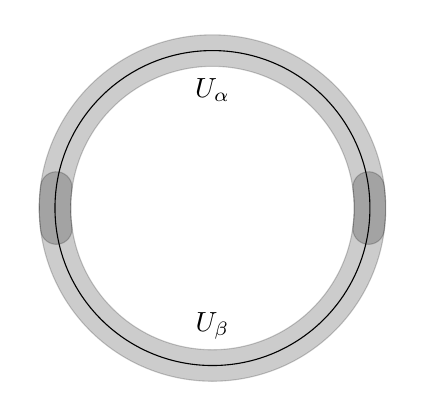
\begin{tikzpicture}
\tikzmath{\overlap=7.5;}

\draw (0,0) circle(2);

\foreach \s/\e in {-\overlap/180 + \overlap, 180 - \overlap/360 + \overlap}
	\draw[fill, opacity=0.2] ([shift=(\s:1.8)]0,0) arc (\s:\e:1.8) arc (180 + \e:\e:0.2) arc (\e:\s:2.2) arc (360 + \s:180 + \s:0.2);
% \coordinate (p0) at (-1.85, -0.0);
% \draw[fill, opacity=0.2]
% 	(-2, +0.2)
% 	to
% 	[
% 		closed,
% 		in curl=.1,
% 		curve through =
% 		{
% 			(p0)
% 			([in angle=90]0.1, -2.0)
% 		}
% 	]
% 	(-2.15, -0.05);

% \draw[fill, opacity=0.2]
% 	(-2, +0.2)
% 	to
% 	[
% 		closed,
% 		in curl=.1,
% 		curve through =
% 		{
% 			(-1.85, -0.0)
% 			(0, -1.8)
% 			(1.85, -0.0)
% 			(2, +0.2)
% 			(2.15, -0.05)
% 			(0, -2.2)
% 						% (0, -1.2)
% 			% (0, -1.2)
% 		}
% 	]
% 	(-2.15, -0.05);
\draw (0, 1.5) node {$U_\alpha$};
\draw (0, -1.5) node {$U_\beta$};
\end{tikzpicture}
\end{document}
